% Copyright (C) Huawei Technologies Co., Ltd. 2024. All rights reserved.
% SPDX-License-Identifier: MIT
\begin{frame}<\theframerange>{As the hardware evolves, so does the concurrency control}
    \begin{columns}
        \column{.6\textwidth}{%
            \begin{block}{Challenges of modern hardware}
                \begin{itemize}\small
                    \item Many-cores everywhere
                    \item<2-> Weak Memory Models, \eg, RISC-V, ARMv8
                    \item<5-> Deep NUMA hierarchies
                    \item<6-> Heterogeneous cores, \eg, big.LITTLE
                \end{itemize}
            \end{block}
        \uncover<7->{%
        \begin{block}{Consequences to concurrent software}
            \begin{itemize}\small
                \item<1-> {Smarter} concurrency is more complex
                \item<8-> {Complexity gets out of control!}
                \item<8-> {\bf Safety compromised:}\\
                    crashes, data corruption, \ldots
            \end{itemize}
        \end{block}}
        }\column{.4\textwidth}{%
            \centering
            \resizebox{\textwidth}{!}{%
            \tikz[align=center,
                n/.style = {ultra thick, line width = 1mm, font=\Large, draw=black, rounded corners, fill=grayish, minimum width=3cm},
                a/.style = {->, line width=2mm},
                news/.style = {draw, very thick, inner sep = 0},
            ]{%
                \draw[use as bounding box, draw=none, dotted] (-5mm, -100mm) rectangle (120mm, 10mm);

                \node<1->[n, fill=blueish] at (-10mm, 10mm)   (hw)  {Multicore\\CPUs};
                \node<1> [right=5mm of hw, yshift=-15mm] (num) {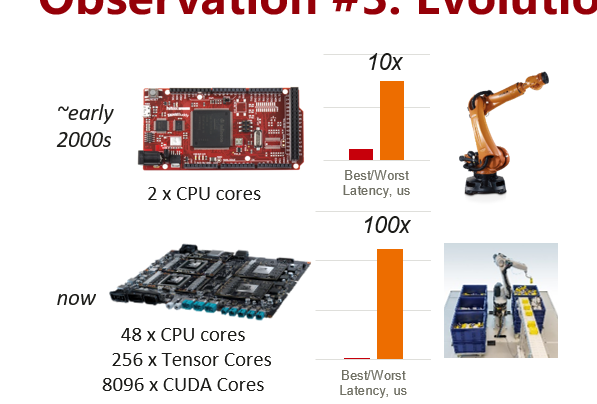
\includegraphics[width=120mm, clip, trim=0 0 0 20]{figs/hardware-evolution.png}};
                \node<2->[right=10mm of hw, yshift=2mm] (num) {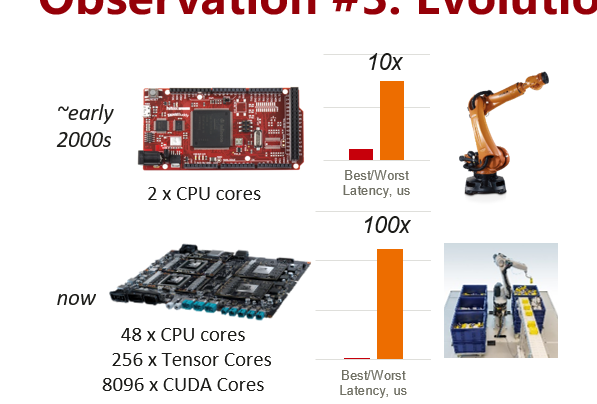
\includegraphics[width=60mm, clip, trim=0 0 0 20]{figs/hardware-evolution.png}};

                \node<2->[n, fill=orangeish, below=35mm of hw] (sw)  {Weak\\Memory};
                \draw<2->[a] (hw) -- (sw);

                \node<3- >[right=10mm of sw] (mp) {\scalebox{1.2}{% Copyright (C) Huawei Technologies Co., Ltd. 2024. All rights reserved.
% SPDX-License-Identifier: MIT
\begin{tikzpicture}[
    a/.style = {->, thick},
    j/.style = {fill=white, font=\scriptsize\bf},
    b/.style = {rounded corners, align=left}, %, text width = 7mm},
    i/.style = {b},
    t/.style = {b, fill=light gray},
    c/.style = {b, fill=light red, text width=34mm},
    ]
\coordinate (x);
\node[i, above=10mm of x] (a) {\verb|msg = 0; ready = false;|};
\node[t, left=5mm of x] (b1) {\verb|msg = 42;|\\ \verb|ready = true;|};
\node[t, right=0mm of x] (b2) {\verb|while(!ready) {}|\\{\verb|assert(msg == 42);|}};
%\node[c, below=of x] (c) {\verb+assert(a != 0 || b != 0);+};
%\draw[a]  (a) -- (b1);
%\draw[a]  (a) -- (b2);
%\draw[a]  (b1) -- (c);
%\draw[a]  (b2) -- (c);
%\node[j, below=1mm of a] {{\tt pthread_create}};
%\node[j, above=1mm of c] {{\tt pthread_join}};
\node[j, above=0 of a] {Init};
\node[j, fill=none, above=0 of b1] (t1) {Thread 1};
\node[j, fill=none, above=0 of b2] (t2) {Thread 2};
\node[text=HuaweiRed, right=-2mm of b2.south east, yshift=2.5mm] {\xmark};

%\draw[a]  (a) -- (t1);
%\draw[a]  (a) -- (t2);
\draw<1->[<->, very thick, HuaweiRed] (b1.170) to [out=180, in = 90]
node[midway, left=1mm, align=center, font=\scriptsize] {WMM\\reorder}
+(-4mm, -2mm) to [out = -90, in = 180] (b1.190);
\end{tikzpicture}
}};

                \node<4->[n, fill=greenish, below=35mm of sw] (alg)  {Heterogeneous\\Cores/Memory};
                \draw<4->[a] (sw) -- (alg);

                \node<5->[right=20mm of alg] (num) {\resizebox{90mm}{!}{% Copyright (C) Huawei Technologies Co., Ltd. 2024. All rights reserved.
% SPDX-License-Identifier: MIT
\begin{tikzpicture}[myarrow/.style={double arrow, draw=none},
  sysbase/.style = {rounded corners, font=\bf, align=left, anchor=center},
    system/.style = {sysbase, draw, dashed},
    proc/.style = {sysbase, fill=grayish, solid, very thick, minimum width=4cm},
    numa/.style = {sysbase, fill=blueish, minimum width=1cm},
    core/.style = {sysbase, fill=white, minimum width=20mm, align=left},
    ]

  \node[system] (nsys) {%
    \begin{tikzpicture}
      \node[proc] (p1) {
        Processor 1\\[4pt]
        \begin{tikzpicture}
          \node[numa] (n1) {Numa 1\\[4pt]
            \begin{tikzpicture}
              \node[core] (c1) {Core 1};
              \node[core, below=1mm of c1] (c2) {Core 2};
              \node[core, below=1mm of c2] (c3) {Core 3};
              \node[core, below=1mm of c3] (c4) {Core 4};
            \end{tikzpicture}
          };
          \node[numa, right=2mm of n1]{Numa 2\\[4pt]
              \begin{tikzpicture}
                \node[core] (c1) {Core 5};
                \node[core, below=1mm of c1] (c2) {Core 6};
                \node[core, below=1mm of c2] (c3) {Core 7};
                \node[core, below=1mm of c3] (c4) {Core 8};
              \end{tikzpicture}
          };
        \end{tikzpicture}
      };
      \node[proc, right=2mm of p1] (p2) {
        Processor 2\\[4pt]
        \begin{tikzpicture}
          \node[numa] (n1) {Numa 2\\[4pt]
            \begin{tikzpicture}
              \node[core] (c1) {Core 9~};
              \node[core, below=1mm of c1] (c2) {Core 10};
              \node[core, below=1mm of c2] (c3) {Core 11};
              \node[core, below=1mm of c3] (c4) {Core 12};
            \end{tikzpicture}
          };
          \node[numa, right=2mm of n1]{Numa 3\\[4pt]
              \begin{tikzpicture}
                \node[core] (c1) {Core 13};
                \node[core, below=1mm of c1] (c2) {Core 14};
                \node[core, below=1mm of c2] (c3) {Core 15};
                \node[core, below=1mm of c3] (c4) {Core 16};
              \end{tikzpicture}
          };
        \end{tikzpicture}
        };
    \end{tikzpicture}
  };
  \node[above=3mm of nsys.north, anchor=center]{Many-core NUMA System};

  \draw<1->[<->, ultra thick, rounded corners, pltgreen,line width=4pt ]
  ($(nsys.north west) + (5mm,-16mm)$)
  to [bend right]
  node[midway, below left=-2mm and 4mm, font=\bf\huge, text=pltgreen, rounded corners] {fast}
  +(-8mm,-3.5mm)
  to [bend right]
  ($(nsys.north west) + (5mm,-23mm)$)
  ;

  \draw<1->[<->, ultra thick, rounded corners, pltred,line width=4pt ]
  ($(nsys.north west) + (38mm,-38mm)$)
  to [out=-90, in=-90]
  node[midway, below=0mm, font=\bf\huge, text=pltred, rounded corners] {slow}
  %+(15mm,-10mm)
  %to [out=0, in=-90]
  ($(nsys.north west) + (68mm,-38mm)$)
  ;

\end{tikzpicture}

}};
                \node<6->[above=-22mm of num.south west, xshift=5mm] {
\includegraphics[width=6cm]{figs/fast-car.png}};
                \node<6->[above=1mm of num.south east] {
\includegraphics[width=2cm]{figs/bike.png}};

                \node<8->[below left=0mm and 2mm of alg] (boom){
\includegraphics[width=50mm]{figs/explosion.png}};
                \draw<8->[a, decorate, decoration={snake, post length=4mm, segment length = 5mm, amplitude = .5mm }] (alg) to[out=-90, in=0] (boom);

            }
            }
        }
    \end{columns}
\end{frame}
